\section{第7讲\quad 综合}

\item {
    【综合;推理】现在有一台奇怪的电脑,电脑上有个按键,如果电脑上原来的数是3的倍数,按下键后就会除以3;如果电脑上原来的数不是3的倍数,那么按下键后就会乘以6.小明在按键前没有看屏幕上的数,结果连按6次,最后电脑上显示的数是12,那么电脑上最开始的数最小可能是\underline{\hbox to 20mm{}}.
    \ifshowSolution
        \fangsong\zihao{4}
        \\
        思路:

        正解: 27
    \else
        \\ \\ \\
    \fi
}

% \item {
%     【数字谜】
%     在右面的乘法竖式中,相同的汉字代表相同的数字,不同的汉字代表不同的数字;那么,\myoverline{迎接夏天} 代表的四位数是\underline{\hbox to 20mm{}}.
%     \begin{figure}[H] 
%         \centering
%         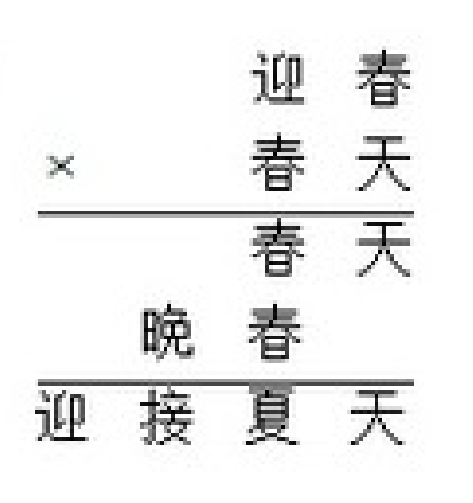
\includegraphics[width=0.4\textwidth]{./pics/Chapter_7/14.png}
%     \end{figure}
%     \vspace{1cm}
%     % 2021; 1024
% }